\documentclass[12pt,a4paper]{article}

% Encoding and font setup
\usepackage[utf8]{inputenc}
\usepackage[T1]{fontenc}
\usepackage{mathptmx} % Times font with math support
\usepackage{microtype} % Better typography

% Geometry and spacing
\usepackage{geometry}
\geometry{a4paper, margin=0.8in}
\usepackage{setspace}
\onehalfspacing

% Math packages
\usepackage{amsmath, amssymb, amsthm, mathtools, bm}

% Hyperlinks
\usepackage{hyperref}
\hypersetup{
    colorlinks=true,
    linkcolor=blue,
    citecolor=blue,
    urlcolor=blue
}

% Lists and formatting
\usepackage{enumitem} % better lists
\usepackage{tocloft}  % customize ToC

% Figures and diagrams
\usepackage{graphicx}
\usepackage{xcolor}
\usepackage{tikz}
\usetikzlibrary{positioning, shapes, arrows, shadows}

% Theorem environments
\theoremstyle{definition}
\newtheorem{definition}{Definition}[subsection]
\newtheorem{theorem}{Theorem}[subsection]
\newtheorem{lemma}{Lemma}[subsection]
\newtheorem{proposition}{Proposition}[subsection]
\newtheorem{remark}{Remark}[subsection]

% Common math shortcuts (minimal set)
\newcommand{\R}{\mathbb{R}}
\newcommand{\vect}[1]{\bm{#1}}
\newcommand{\norm}[1]{\left\lVert #1 \right\rVert}

% Title page
\begin{document}

\begin{titlepage}
    \centering
    \vspace*{1cm}
    {\huge \textbf{From Projection to Perception: \\ A Mathematical Exploration of \\ Shadow-based Neural Reconstruction}\par}
    \vspace{1.5cm}
    {\normalsize
    A research report submitted to the Scientific Committee of the Hang Lung Mathematics Award\par}
    \vspace{1cm}
    {\normalsize \textbf{Team Number}\par 2596873\par}
    \vspace{0.5cm}
    {\normalsize \textbf{Team Members}\par Wong Yuk To, Hung Kwong Lam \\ Cheung Tsz Lung, Chan Ngo Tin, Zhou Lam Ho\par}
    \vspace{0.5cm}
    {\normalsize \textbf{Teacher}\par Mr. Chan Ping Ho\par}
    \vspace{0.5cm}
    {\normalsize \textbf{School}\par Po Leung Kuk Celine Ho Yam Tong College\par}
    \vspace{0.5cm}
    {\normalsize \textbf{Date}\par \today\par}
    \vfill

    \begin{abstract}
    \noindent
    This paper explores \textsc{ShadowNeuS} \hyperlink{[LWX23]}{[LWX23]}, a neural network that reconstructs 3D geometry from single-view camera images using shadow and light cues. Unlike traditional 3D reconstruction methods relying on multi-view cameras or sensors, \textsc{ShadowNeuS} leverages a neural signed distance field (SDF) for accurate 3D geometry reconstruction. We analyze the training process and uncover its connections to projective geometry, spatial reasoning in $\R^3$, and the neural network's learned geometric representation of space.
    \end{abstract}
\end{titlepage}

\tableofcontents
\newpage

\section{Introduction}
\subsection{Background}
3D reconstruction is the process of recovering the shape and structure of an object in \(\mathbb{R}^3\) from measured data. It has broad applications in medical imaging (MRI, CT), robotics, augmented/virtual reality (AR/VR), and cultural heritage preservation. Most conventional methods rely heavily on geometric and physical modeling techniques and require rich spatial data obtained through multi-view camera setups, LiDAR sensors, or photogrammetry.

\subsection{Motivation}
Traditional approaches typically depend on \textbf{multiple viewpoints or depth sensors}, which is costly and complex. This leads to the question: \textbf{Is it possible to reconstruct 3D geometry from a single fixed camera?} A single image inherently lacks depth information, and multiple 3D points can project to the same 2D pixel location (as discussed in Section \ref{sec: illposed}). Therefore, additional cues are essential to resolve this ambiguity. \\
In exploring this problem, we discovered the paper \textit{ShadowNeuS: Neural SDF Reconstruction by Shadow Ray Supervision} \hyperlink{[LWX23]}{[LWX23]} by Jingwang Ling, Zhibo Wang, and Feng Xu. Their approach demonstrates that leveraging neural signed distance fields and supervising the network with shadow ray information under varying lighting enables accurate 3D reconstruction from single-view images. Motivated by their work, we present a study analyzing their method and propose a 1D-to-2D experimental validation to examine our understanding.

\section{Fundamentals of 3D Reconstruction from 2D Images}
\subsection{3D Reconstruction in Computer Vision}
According to an article on Medium \hyperlink{[VK23]}{[VK23]}, 3D computer vision is a field of computer science focusing on the analysis, interpretation, and understanding of three-dimensional visual data. \\
The article highlights a traditional approach for 3D reconstruction:

\begin{minipage}{0.5\textwidth}
    \textbf{Structure from Motion (SfM)} \\
    Recover the 3D structure by estimating camera \\ positions from multiple images.
\end{minipage}
\hspace{0.5cm}
\begin{minipage}{0.5\textwidth}
    \centering
    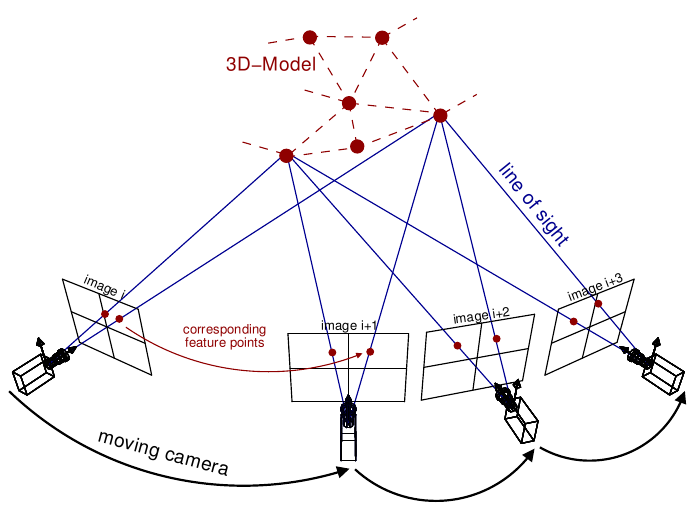
\includegraphics[height=0.2\textheight]{SfM.png} \\
    \hyperlink{[Fig 1]}{\textbf{Figure 1.}} Structure from Motion
\end{minipage}

\newpage

\subsection{Information Encoded in a Single-View Image}
When only single-view is available, the following information remains exploitable:

\begin{itemize}[noitemsep, topsep=0pt, parsep=0pt, partopsep=0pt]
    \item \textbf{Pixel position \((u, v)\)} — relates to a 3D ray from camera to that pixel
    \item \textbf{Color / intensity} — encodes surface information (material, orientation, etc.)
    \item \textbf{Embedded features} (edges, recognized objects) — encode geometry cues
\end{itemize}

\begin{center}
\begin{minipage}{0.35\textwidth}
    \centering
    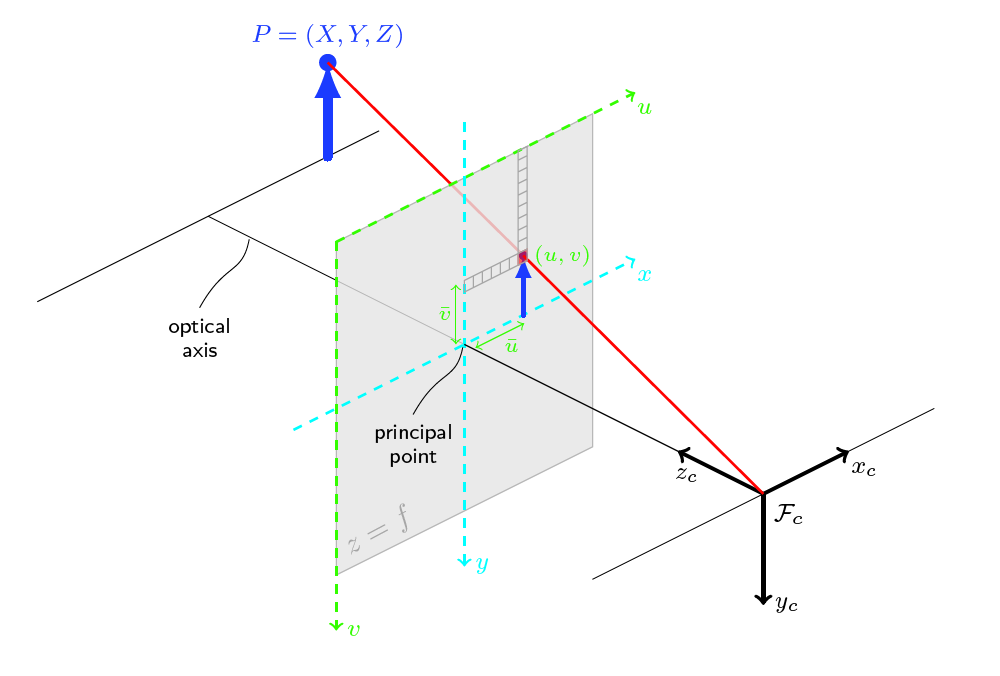
\includegraphics[width=\textwidth]{pixel_position.png} \\
    \hyperlink{[Fig 2]}{\textbf{Figure 2.}} Ray from camera to pixel
\end{minipage}
\hfill
\begin{minipage}{0.2\textwidth}
    \centering
    
\includegraphics[width=\textwidth]{color_intensity.jpg} \\
    \hyperlink{[Fig 3]}{\textbf{Figure 3.}} Texture
\end{minipage}
\hfill
\begin{minipage}{0.35\textwidth}
    \centering
    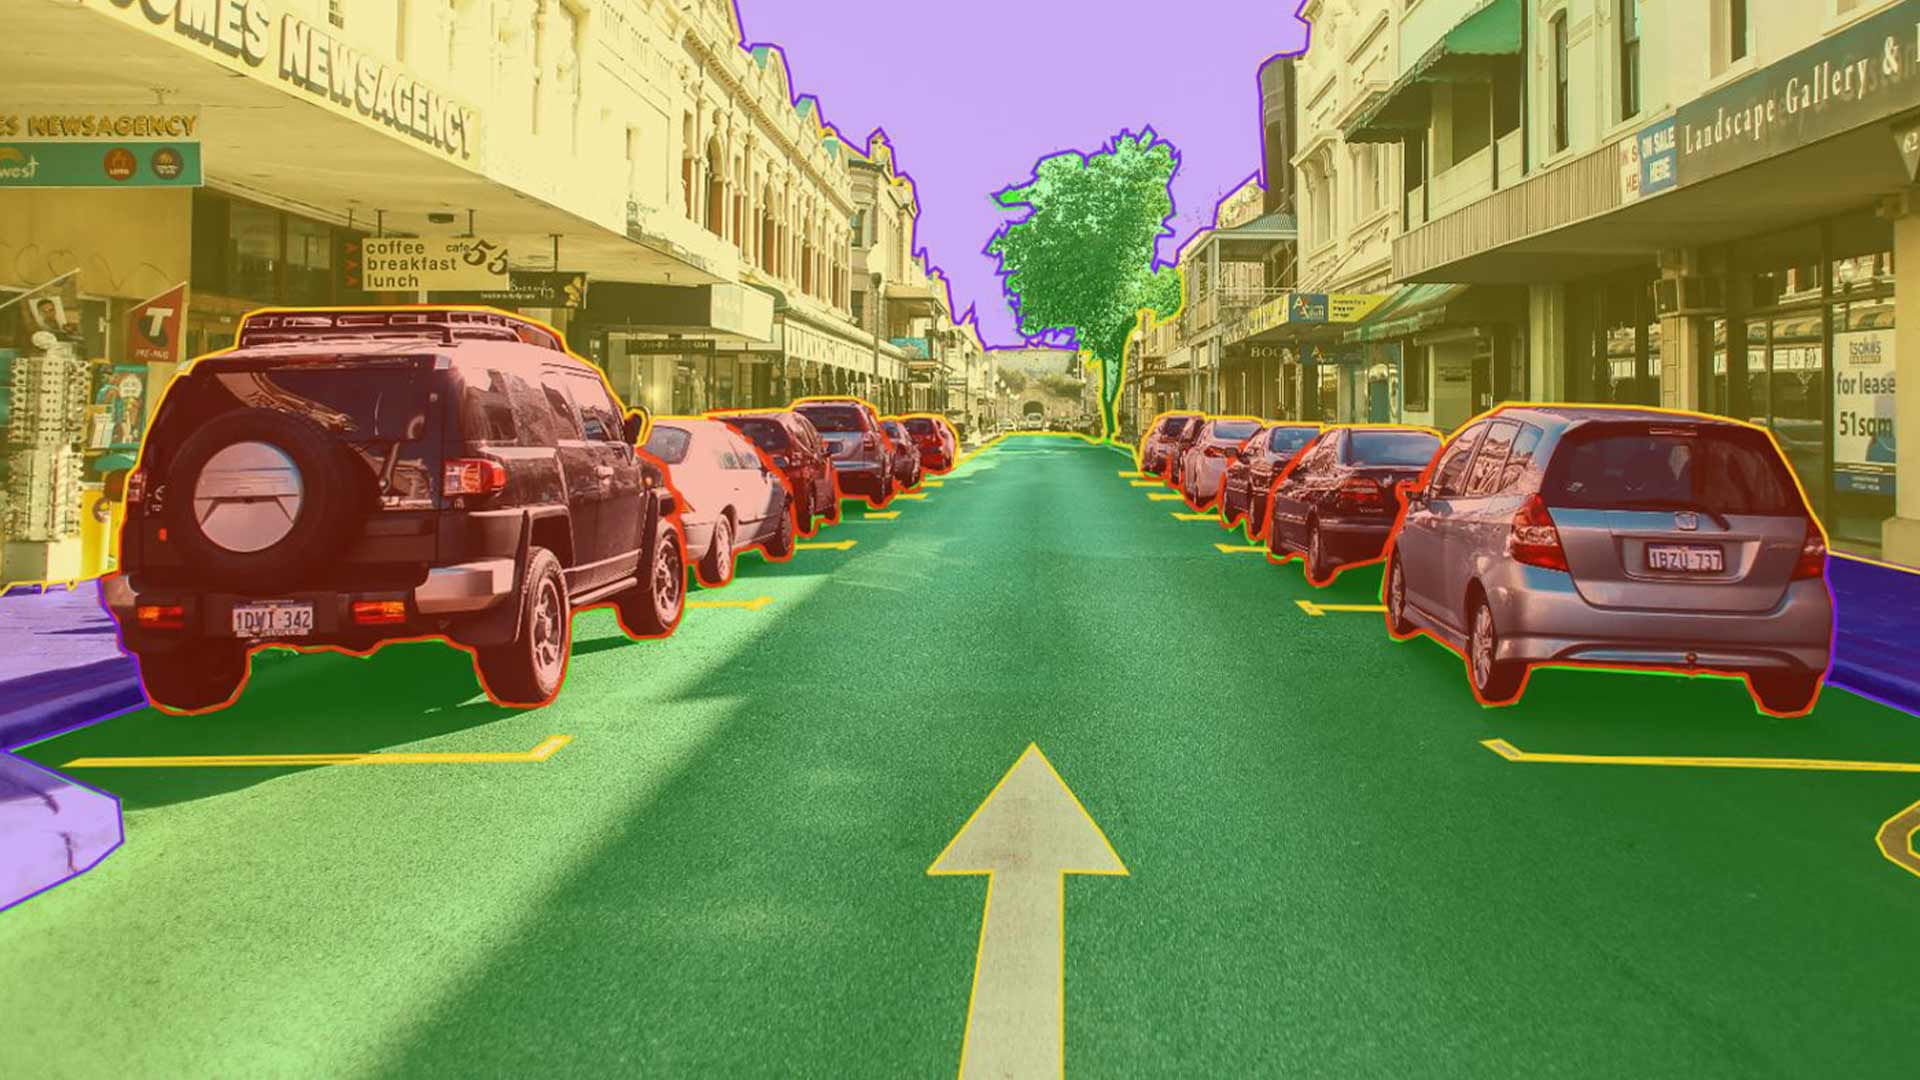
\includegraphics[width=\textwidth]{embedded_features.jpg} \\
    \hyperlink{[Fig 4]}{\textbf{Figure 4.}} Object segmentation (YOLO)
\end{minipage}
\end{center}

\vspace{-1em}

\subsection{Forward Projection: Mapping from 3D to 2D} \label{sec:forward_projection}
\vspace{-0.5em}
In this section, we want to show that mapping from a 3D point \(\vect{P} = (x,y,z)^\mathsf{T} \in \R^3\) in the world coordinate system onto a 2D image pixel coordinate \(\vect{p} = (u,v)^\mathsf{T} \in \R^2\) is a projection-like process.

\noindent\textbf{Extrinsic parameters:} define the camera's position and orientation relative to the world:
\vspace{-0.5em}
\begin{equation}
C = \underbrace{\begin{bmatrix} C_x \\ C_y \\ C_z \end{bmatrix} \in \R^3}_{\substack{\text{Camera center}}}, \quad
R = \underbrace{
\begin{bmatrix}
r_{11} & r_{12} & r_{13} \\
r_{21} & r_{22} & r_{23} \\
r_{31} & r_{32} & r_{33}
\end{bmatrix} \in \mathrm{SO}(3)
}_{\substack{\text{Rotation matrix}}}, \quad
t = \underbrace{-R C \in \R^3}_{\substack{\text{Translation vector}}}
\label{eq:extrinsic}
\end{equation}

\noindent\textbf{Intrinsic parameters:} encode the internal camera geometry:
\vspace{-0.5em}
\begin{equation}
K = \begin{bmatrix}
f_x & 0 & c_x \\
0 & f_y & c_y \\
0 & 0 & 1
\end{bmatrix} \in \R^{3 \times 3}
\label{eq:intrinsic}
\end{equation}
where \((f_x, f_y)\) are the focal lengths in pixels, and \((c_x, c_y)\) is the principal point (image center).

The forward projection consists of three steps:
\begin{enumerate}[noitemsep, topsep=0pt, parsep=0pt, partopsep=0pt]
    \item Transform \(\vect{P}\) from world coordinates to camera coordinates: \(\vect{P}_{\text{cam}} = R (\vect{P} - C) = R \vect{P} + t\).
    \item Project camera coordinates to homogeneous image coordinates: \(\vect{P}_{\text{hom}} = K \vect{P}_{\text{cam}} = \begin{bmatrix} p_x' \\ p_y' \\ z' \end{bmatrix}\).
    \vspace{-0.5em}
    \item Normalize by depth \(z'\) to get pixel coordinates: \(\vect{p} = \frac{1}{z'} \begin{bmatrix} p_x' \\ p_y' \end{bmatrix}, \quad z' \neq 0\).
\end{enumerate}

Combined expressions:
\begin{equation}
\boxed{
\vect{P}_{\text{hom}} = \begin{bmatrix} p_x' \\ p_y' \\ z' \end{bmatrix} = K [R \mid t] \begin{bmatrix} \vect{P} \\ 1 \end{bmatrix}, \quad
\vect{p} = \frac{1}{z'} \begin{bmatrix} p_x' \\ p_y' \end{bmatrix}
}
\label{eq:forward}
\end{equation}

\newpage

\subsection{The Inverse Problem: From 2D Image to 3D World} \label{sec:inverse_problem}

After understanding the forward projection process, 3D reconstruction can be viewed as the inverse calculation: recovering 3D points from their 2D image projections. \\  
We now tackle the challenge of inverting the projection function introduced in Section \ref{sec:forward_projection}.

\begin{lemma}[Camera Ray Parametrization] \label{lem:camera_ray} ~\\
Given a pixel \(p = [p_x, p_y]^\mathsf{T}\) and camera parameters \((K, R, C)\), the corresponding 3D points lie on a ray:
\begin{equation}
\boxed{P(\lambda) = C + \lambda \, d, \quad \lambda > 0}
\end{equation}
where the ray direction is
\begin{equation}
\boxed{d = R^{-1} K^{-1} \begin{bmatrix} p_x \\ p_y \\ 1 \end{bmatrix}}
\end{equation}
\begin{remark}[Normalization] ~\\
The vector \(d\) can be normalized to unit length for physical interpretation, but this is not essential for the ray parametrization.
\end{remark}
\end{lemma}

\begin{proof}
Starting from the forward projection \eqref{eq:forward}:
\begin{align*}
K (R P + t) &= z' \begin{bmatrix} p_x \\ p_y \\ 1 \end{bmatrix}, \\
R P + t &= z' K^{-1} \begin{bmatrix} p_x \\ p_y \\ 1 \end{bmatrix}, \\
P &= R^{-1} \bigl(z' K^{-1} \begin{bmatrix} p_x \\ p_y \\ 1 \end{bmatrix} - t \bigr).
\end{align*}
Since \(t = -R C\), we have \(-R^{-1} t = C\). Setting \(\lambda = z'\), the parametric form of the ray follows:
\[
P(\lambda) = C + \lambda \, R^{-1} K^{-1} \begin{bmatrix} p_x \\ p_y \\ 1 \end{bmatrix}.
\]
\end{proof}

By parametrizing the ray originating at \(C\) in the direction \(d\), we capture the geometric meaning that a single pixel in an image does not correspond to a unique 3D point but rather to an infinite set of points lying along this ray.

\newpage

\subsection{Ill-posedness and Ambiguity in Single-View Reconstruction} \label{sec: illposed}
\vspace{-0.5em}
Recovering 3D points from a single 2D image is \textbf{ill-posed}, as defined by Hadamard: the solution may be non-unique, unstable, or nonexistent.
\vspace{-0.5em}
\begin{proposition}[Ill-posed Nature of Single-View Reconstruction]~\
\begin{enumerate}[label=(\alph*), noitemsep, topsep=0pt, parsep=0pt, partopsep=0pt]
    \item The depth \(\lambda\) is unknown.
    \item Each pixel \(\vect{p}\) corresponds to infinitely many 3D points along a ray.
    \item Additional constraints are needed for unique reconstruction.
\end{enumerate}
\end{proposition}

This ill-posedness motivates using extra cues like multiple views (SfM), depth sensors, or shadow information.
\vspace{-1.5em}

\section{Shadows as Geometric Constraints}
\vspace{-1em}
To what extent can shadows constrain 3D geometry from a single image? In this section, we will explore how shadows form from interaction of light and geometry, how these shadows partition the 3D surface and the 2D image, and how this partitioning can help recover depth information. 
\vspace{-1em}

\subsection{Light Rays and Shadow Formation due to Blockage}
\begin{definition}[Light Ray] \label{def:light_ray} ~\\
Given a point light source $\vect{L} \in \R^3$ and a surface point $\vect{P} \in \R^3$, the light ray is:
\begin{equation}
\boxed{r(t) = \vect{L} + t(\vect{P} - \vect{L}), \quad t \in [0,1]} \label{eq:light_ray}
\end{equation}
\end{definition}

\begin{definition}[Shadow Occlusion Test] \label{def:shadow_occlusion} ~\\
A point $\vect{P}$ is in shadow if there exists $t \in (0,1)$ such that the light ray intersects a surface $\mathcal{S}$:
\begin{equation}
\boxed{r(t) \cap \mathcal{S} \neq \emptyset, \quad t \in (0,1)}
\end{equation}
\end{definition}

\begin{remark}[Physical Interpretation] \label{rmk:occlusion_physics} ~\\
The interval $(0,1)$ excludes the light source ($t=0$) and the target point ($t=1$), ensuring the test checks for obstructions between $\vect{L}$ and $\vect{P}$. This models physical light transport where occlusion by another surface causes a shadow.
\end{remark}

\vspace{-3em}
\begin{center}
    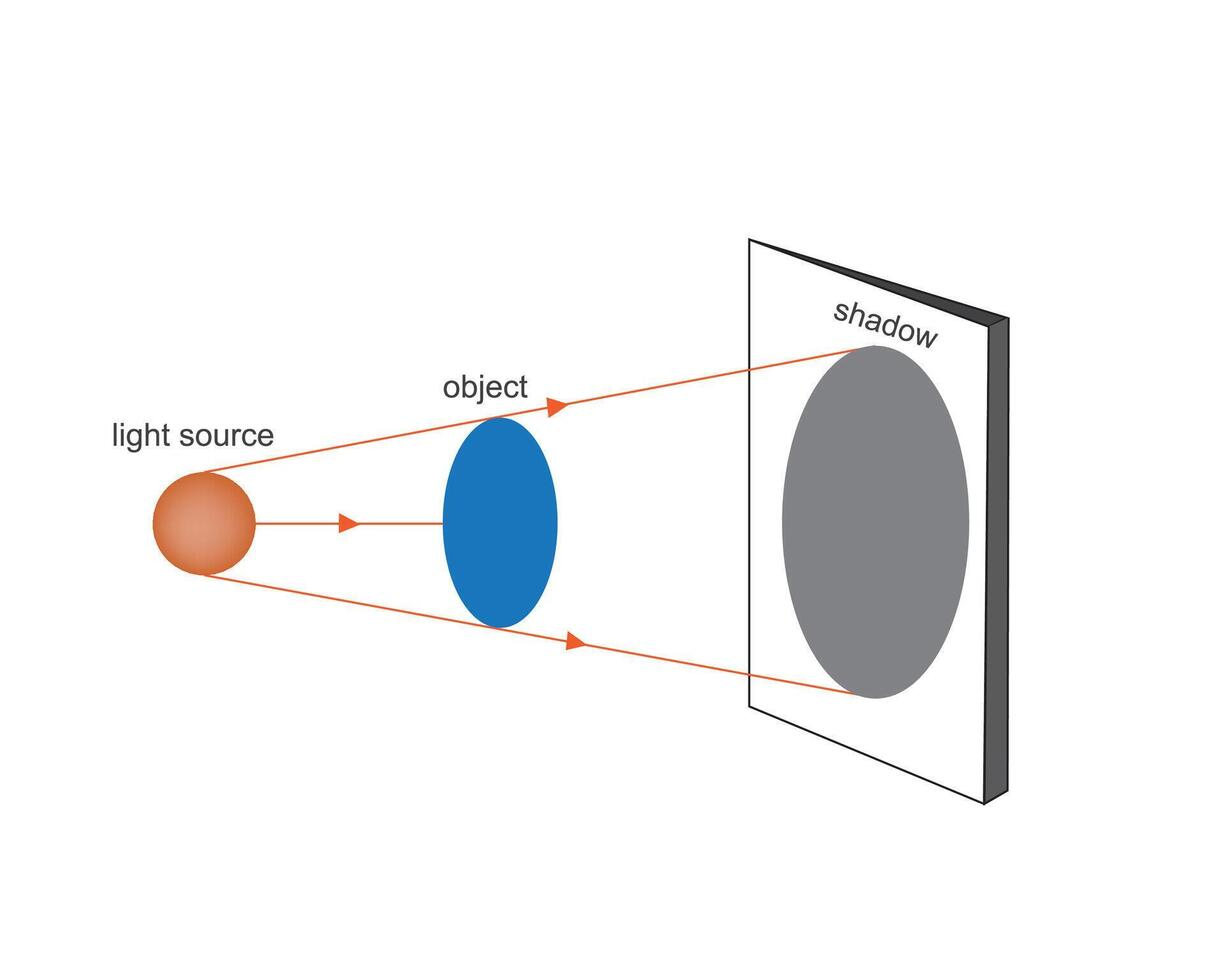
\includegraphics[width=0.5\textwidth]{shadow-of-object-vector.jpg} \\
    \hyperlink{[Fig 5]}{\textbf{Figure 5.}} Shadow Formation due to Blockage
\end{center}

\newpage


\subsection{Surface Normals and Shadow Formation due to Orientation}
\vspace{-0.5em}
\begin{theorem}[Tangency Condition] \label{thm:tangency} ~\\
A point \(\vect{Q} \in \mathcal{S}\) lies on the shadow boundary if and only if the light direction at \(\vect{Q}\) is tangent to the surface:
\begin{equation}
\boxed{(\vect{Q} - \vect{L}) \cdot \vect{n}(\vect{Q}) = 0} \label{eq:tangency}
\end{equation}
where \(\vect{n}(\vect{Q})\) is the outward unit normal vector at \(\vect{Q}\).
\end{theorem}

\begin{proof}
At the shadow boundary, the light ray \(r(t)\) just grazes the surface \(\mathcal{S}\) at \(\vect{Q}\). This means the vector from the light source to \(\vect{Q}\), \(\vect{Q} - \vect{L}\), lies in the tangent plane of \(\mathcal{S}\) at \(\vect{Q}\). Since the tangent plane is orthogonal to the surface normal \(\vect{n}(\vect{Q})\), their dot product is zero: $(\vect{Q} - \vect{L}) \cdot \vect{n}(\vect{Q}) = 0$
\end{proof}

\begin{definition}[Shadow Boundary Set] \label{def:boundary_set} ~\\
The 3D shadow boundary \(\mathcal{B}\) consists of all points on \(\mathcal{S}\) where the light direction is tangent:
\begin{equation}
\boxed{\mathcal{B} = \{\vect{Q} \in \mathcal{S} \mid (\vect{Q} - \vect{L}) \cdot \vect{n}(\vect{Q}) = 0\}} \label{eq:boundary_set}
\end{equation}
\end{definition}

\begin{proposition}[Surface Illumination Partition] \label{prop:illumination_partition} ~\\
The surface \(\mathcal{S}\) is divided into three disjoint regions based on the sign of the dot product between the light direction and surface normal:
\begin{align}
\mathcal{S}_{\text{lit}} &= \{\vect{P} \in \mathcal{S} \mid (\vect{P} - \vect{L}) \cdot \vect{n}(\vect{P}) > 0\} && \text{(illuminated region)} \label{eq:lit_region} \\
\mathcal{S}_{\text{shadow}} &= \{\vect{P} \in \mathcal{S} \mid (\vect{P} - \vect{L}) \cdot \vect{n}(\vect{P}) < 0\} && \text{(attached shadow region)} \label{eq:shadow_region} \\
\mathcal{B} &= \{\vect{P} \in \mathcal{S} \mid (\vect{P} - \vect{L}) \cdot \vect{n}(\vect{P}) = 0\} && \text{(shadow boundary)} \label{eq:boundary_region}
\end{align}
\end{proposition}

\begin{remark}[Geometric Interpretation] \label{rmk:illum_sign} ~\\
The sign of the dot product \((\vect{P} - \vect{L}) \cdot \vect{n}(\vect{P})\) encodes the relative angle between the surface normal and the direction to the light source. Positive values indicate the surface faces toward the light (lit), negative values indicate it faces away (shadowed), and zero indicates a tangent point forming the shadow boundary.
\end{remark}
























\section{ShadowNeuS: Neural SDF Reconstruction by Shadow Ray Supervision}
% ...

\section{Experimental Demonstration}
% ...

\section{Discussion and Analysis}
% ...

\section{Conclusion}
% ...


\section*{References}
\spaceskip=0.3em plus 0.1em minus 0.1em
\begin{tabular}{p{0.15\textwidth}p{0.85\textwidth}}
{[LWX23]}               & Jingwang Ling, Zhibo Wang, Feng Xu. \textit{ShadowNeuS: Neural SDF Reconstruction by Shadow Ray Supervision}. arXiv: \href{https://arxiv.org/abs/2211.14086}{2211.14086}, 2023. \hypertarget{[LWX23]}{}  \\
{[VK23]}                & Venkatkumar. \textit{3D Reconstruction Basic Terminology (Traditional Computer Vision Approach)}. Medium: \href{https://medium.com/@VK_Venkatkumar/3d-reconstruction-basic-terminology-traditional-computer-vision-e148496f389}{URL}, 2023. \hypertarget{[VK23]}{} \\
{[\textbf{Figure 1.}]}  & Sjoerd van Riel. \textit{Exploring the use of 3D GIS as an analytical tool in archaeological excavation practice}. ResearchGate: \href{https://www.researchgate.net/figure/Structure-from-Motion-SfM-photogrammetric-principle-Source-Theia-sfmorg-2016_fig3_303824023}{URL}, 2016. \hypertarget{[Fig 1]}{} \\
{[\textbf{Figure 2.}]}  & Catree. \href{https://stackoverflow.com/questions/38494485/camera-coordinate-to-pixel-coordinate-opencv}{Camera coordinate to pixel coordinate - OpenCV}, 2016. \hypertarget{[Fig 2]}{} \\
{[\textbf{Figure 3.}]}  & Lemanoosh. \href{https://lemanoosh.com/online-course-blender-material-rendering/}{Blender material rendering}, n.d. \hypertarget{[Fig 3]}{}  \\
{[\textbf{Figure 4.}]}  & Michael Abramov. \href{https://keymakr.com/blog/semantic-segmentation-vs-object-detection-understanding-the-differences/}{Semantic Segmentation vs Object Detection: Understanding the Differences}, 2024. \hypertarget{[Fig 4]}{}  \\
{[\textbf{Figure 5.}]}  & Sandip Neogi. \href{https://www.vecteezy.com/vector-art/42399612-shadow-of-object}{shadow of object Pro Vector}, n.d. \hypertarget{[Fig 5]}{}  \\
\end{tabular}


\end{document}